% this file is called up by thesis.tex
% content in this file will be fed into the main document

\chapter{Background}\label{ch:background} % top level followed by section, subsection


% ----------------------- paths to graphics ------------------------

% change according to folder and file names
\ifpdf
    \graphicspath{{7/figures/PNG/}{7/figures/PDF/}{7/figures/}}
\else
    \graphicspath{{7/figures/EPS/}{7/figures/}}
\fi


% ----------------------- contents from here ------------------------
%
%
In this section, background information on key value stores, which is the backbone of this thesis, will be given.
Also, the issues with commonly used linux sockets, will be explained.
Further, RDMA is thoroughly explained, as this is crucial to the understanding of this paper, and how it addresses issues facing sockets.

\section[KV-store]{Key Value Store}\label{sec:kv-store}
Key value stores are extensively used to offer low latency look ups.
These have a wide variety of use cases, most notably as cache systems, such as Memcached\cite{memcached}, and as remote DRAM storage, such as RAMCloud\cite{ousterhout2010case}.
In its simplest form, KV store use a set of commands, commonly SET, GET, and DEL, to perform tasks on a server.
These commands interact with a fast data structure, like hash table or similar.
Typically, this was the target for advancements in KV stores, using lower latency, memory efficient, and scalable data structures\cite{lim2014mica, escriva2012hyperdex}.

It has been found that typical work loads consist mostly of GET requests.
Atikoglu et. al. analysed workloads on Memcached systems, and have found that on average a 30:1 (95\%) GET/SET ratio\cite{atikoglu2012workload}.
This figure will be used in the benchmarking design, see section \ref{sec:benchmark-design}.

\section[Linux scokets and TCP]{Linux sockets and TCP network stack}\label{sec:linux-sockets}
Linux sockets are versatile programming API, offering for many types: files, IO, and lastly networking.
Behind this socket interface, the kernel is tasked with data and memory, and connection management\cite{hanford2018survey, seth2009tcp}.
This results in CPU cycles being used to process incoming packets and data copies, while these cycles could be used for other tasks.
Linux takes an extensive route when dealing with packets, as shown by Hanford et. al. detailed investigation\cite{hanford2018survey}.
Memory copies have been found to cause delay in Frey and Alonso's work\cite{frey2009minimizing}, however for small message sizes, Yasukata, and team, found this is insignificant\cite{yasukata2016stackmap}.
TCP processing accounted for more than half of the overhead, after subtracting unavoidable PCIe latencies.

Past attempts at improving TCP performance included offloading most processing to the network interface card (NIC)\cite{hanford2018survey}.
Higher end NICs use an TCP offload engine (TOE) and DMA.
The socket API still requires system calls, among other limitations, thus requiring kernel trapping for management.

\section[RDMA]{RDMA}\label{sec:rdma}
Remote Direct Memory Access (RDMA) address the issues of linux sockets, providing lower latency, less CPU overhead, and potentially higher throughput.
RDMA has been used in super computers for many years, however recently have seen significant improvements.
RDMA capable network cards (RNICs) have seen lowering in cost \cite{kalia2016design}, which made this an appealing improvement to data center networking.

RDMA achieves this low latency by offloading the network processing onto the RNIC, bypassing CPU and kernel entirely.
As shown in section \ref{sec:linux-sockets} above, the linux kernel has an extensive route, from application to NIC to network, including system calls and memory copies.
With RDMA, a zero-copy memory access can be realised through DMA and programmable IO (PIO) operations.
This makes RDMA a compelling technology for latency sensitive workloads, like KV-store, making remote memory operations possible and perform near to local memory operation speeds.

\subsection{Queue Pairs}\label{subsec:queue-pairs}
RDMA is largely based around the notion of a queue pair (QP).
These consist of a send and receive queue, these are the essence of performing network operations.
These queues can be seen as the receive and transmit queue (RX and TX respectively) in classical NIC, however are bound per QP instead of being shared system wide.
A QP is similar to a linux socket, as these are used to send and receive data.
A work request (WR) is a type of command that tells the RNIC what task to perform and which memory locations are needed, these are passed to the RNIC via PIO operations.
For RDMA operations like READ and WRITE this would include the remote address to be accessed, with two-sided verbs such as SEND and RECV this is accompanied by a buffer for which DMA operations can take place.
In this paper, the focus will be on SEND and RECV verbs, more can be read in section \ref{subsec:verbs} below and in \ref{sec:rdma2}.
Every WR placed either in the send or receive queue will be consumed in the same order as placed in the queue, similarly for completions of WR's.
This is important when dealing with unreliable transportation, as will be explained in \ref{subsec:transportation-types}.

Queue pairs are also linked with a completion queue (CQ).
This queue is used as a notification queue, with the status of WR's.
For signalled WR's, a completion event will be passed from RNIC to CPU, thus minor CPU involvement.

\subsection{Transportation types}\label{subsec:transportation-types}
Much like traditional networking, RDMA can make use of several transport protocols.
Simply put, these can be split into two types, connection and datagram, and reliable and unreliable.
There are 3 main transportation types: reliable connection (RC), unreliable connection (UC), and unreliable datagram (UD).

Firstly, unreliable protocols do not make use of ACK/NAK packets, while this is used for reliable, this could result in packet loss and unordered packets.
However, it has been shown that this rarely occurs\cite{kalia2014using, kalia2016fasst}.
Additionally, this could require application retransmission handling.
With reliable protocol this is process is done by the RNIC, without OS or application involvement.

As stated in the name, RC and UC need a connection between queue pairs (QP).
Only one QP can be connected to another QP.
Contrasting this, unreliable datagram (UD) do not require a connection.
This meaning that a UD QP can communicate with any other UD QP.
UD therefore can make efficient use of a one-to-many network topology or application, and RNIC cache.
Every QP has to be held by RNIC in cache, which is severely limited\cite{qiu2018toward}.
A cache miss or many context switching in RNIC, would diminish performance.
With the fan-in and fan-out effect present in many data center workloads\cite{vasudevan2009safe}, the potential scalability of connection oriented QP's is limited\cite{kalia2016fasst}.
UD requires an adress handler (AH) to be passed along with its WR's.
This is the route and the destination for a packet.
The destination does not need to be a QP, but could also be a multicast group.
Multiple clients can listen on the same channel, this is can be applied in applications where the same data can be used by multiple clients.
An AH can be created from a previous work completion (WC), or via metadata exchange, see \ref{subsec:connecting-qp's}.

UD is limited however in the maximum transmission unit (MTU).
As can be seen in table \ref{tab:transport-verb}, UD has a maximum message size of 4KB, beyond this and the message is divided into several packets.
This strongly contrasts the 2 GB available for RC and UC.
This has to be taken into account on a per-application bases.
In the case of this thesis, 4 KB is sufficient message size for KV-stores.
Frey and Alonso have comprised a list of application and if it is suitable for RDMA\cite{frey2009minimizing}.

\subsection{Verbs}\label{subsec:verbs}
To interact with RNICs, RDMA uses so-called "verbs" to execute specific types of instructions.
Some of which are: read, write, send, and receive.
Read and write follow so-called memory semantics, while send and receive follow channel semantics.
Memory semantics require the destination memory address to be known.
This meaning, to be able to perform a RDMA read of a remote memory location, the memory address of the requested memory needs to be known.

Channel semantics are simpler in the sense that the remote memory address does not need to be known.
However, to perform a send operation from client to server, the server needs to first post a receive.
This tells the server's RNIC which memory location the application expects the next incoming message to be place.

Not all verbs are available to every QP type. Table \ref{tab:transport-verb} summarizes the transportation type and which verb is available.

\begin{table}
    \centering
    \begin{tabular}{lllllr}
        \toprule
          & \textbf{SEND} & \textbf{RECV} & \textbf{READ} & \textbf{WRITE} & \textbf{MTU size} \\
        \midrule
        \textit{RC} & YES & YES & YES & YES & 2 GB \\
        \textit{UC} & YES & YES & NO & YES & 2 GB \\
        \textit{UD} & YES & YES & NO & NO & 4 KB \\
        \bottomrule
    \end{tabular}
    \caption{Verbs available to each transportation type}
    \label{tab:transport-verb}
\end{table}

\subsection{Connecting Queue Pairs}\label{subsec:connecting-qp's}
Establishing a connection between QP's involves exchanging metadata related to the QP.
This can be done via a known QP, or via traditional communication like sockets.
The latter is simplest, since it is a well established.
However, in some cases, a classical ethernet is not available.
In these circumstances, a known QP, Communication Manager (CM), can be used.
This is a QP which is always available when using RNIC, and can be used to communicate between RNICs.

Unconnected datagrams also require metadata exchange, despite not being connected.
Data such as QP number, and physical port, which is are needed to create AH, or join a multicast group.
This can be achieved in the same way as with connected protocols.

\subsection{Programming with RDMA}\label{subsec:programming-with-rdma}

\begin{figure}
    \centering
    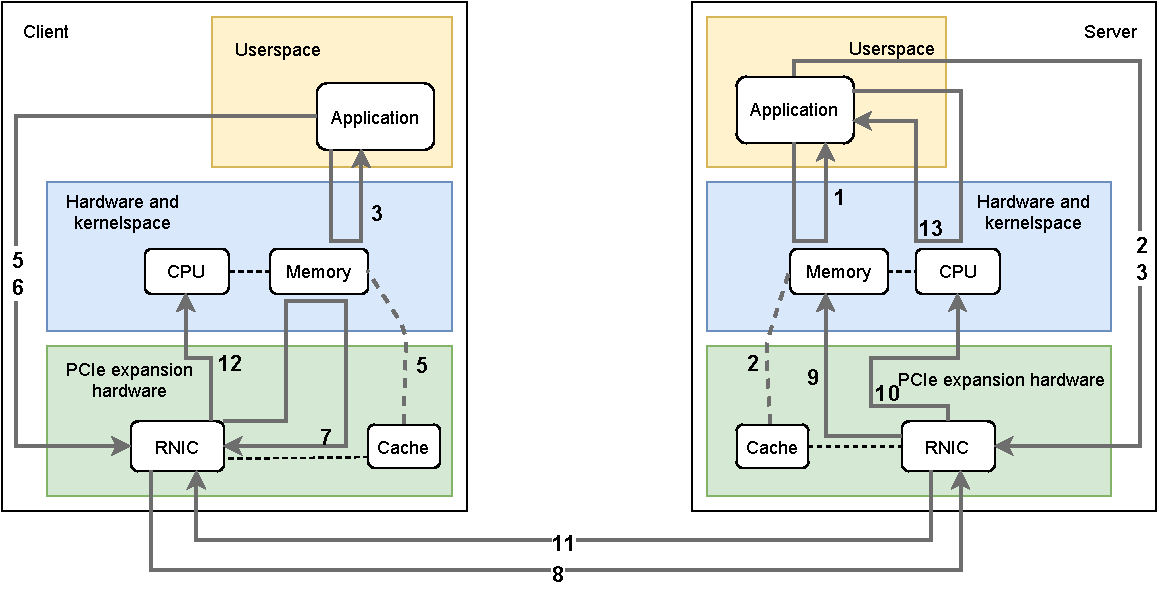
\includegraphics[width=\columnwidth]{figures/PDF/RDAM_SEND_RECV_drawing}
    \caption[Process overview of SEND and RECV.]{Process overview of pre-posting receive and send from client to server. Numbered arrows have a corresponding function described in \ref{subsec:programming-with-rdma}. Numbered dashed lines are cache page entries for registered memory.}
    \label{fig:send_recv_drawing}
\end{figure}

Unlike traditional sockets, much of RDMA's interfacing is open to the programmer, allowing for more detailed optimizations.
The cost of this is the need for more memory management in userspace, which otherwise would be done by the kernel.
In this section, this open interface will be discussed, what functions are needed to be done to make use of RDMA, and what happens internally.
For this, figure \ref{fig:send_recv_drawing} illustrates the process of a send and receive operation, from client to server.
It is assumed that client and server have successfully made a protection domain (PD), QP, and connect or exchanged data for these QP's, see section \ref{subsec:connecting-qp's} on how this can be done.
The numbered arrows in figure \ref{fig:send_recv_drawing} correspond to the following:

\begin{enumerate}
    \item The server application should allocate memory for its receiving buffer.
    \item This buffer should be registered in the RNIC under the PD used for this application.
    By registering memory, a page table entry will be held in RNIC's cache.
    \item Server pre-posts a receive.
    This is needed to be able to receive before the client will send.
    Usually this is done just before connecting, this way even if the receiving end lags behind, the RNIC will be ready to receive.
    \item Client allocates the buffer that will be sent.
    \item Also registering this buffer.
    This can be done while the server is completing steps 1 and 2.
    \item Posting a SEND WR to the RNIC.
    This signals the RNIC that a given registered memory address will be sent via its QP.
    \item The RNIC fetches this data in memory using DMA.
    \item In step 8, this data is then sent over the network to the server.
    \item The server's RNIC receives this data and performs an DMA operation to the buffer given by its RECV WR.
    \item RNIC notifies with a completion event to the CPU, that it has a new event in its CQ.
    \item RNIC also sends an completion event to the client.
    \item This is passed along to the CPU.
    \item The server can poll on the CQ, this tells the application that the RECV request has been completed.
\end{enumerate}


% ---------------------------------------------------------------------------
% ----------------------- end of thesis sub-document ------------------------
% ---------------------------------------------------------------------------